\documentclass[a4paper,10pt]{report} % {article}
%\documentclass[a4paper,10pt]{scrartcl}


% --- input -----------------------------------
  \usepackage[utf8]{inputenc}
  \usepackage[base]{babel} 

% --- math -----------------------------------
  \usepackage{amsmath}
  \usepackage{amsfonts}
  \usepackage{amstext}
  \usepackage{amssymb}
  \usepackage{amsthm}
   

% --- graphic and formating ------------------
  % bibliography
  \usepackage[sort,comma]{natbib} 
  % settings
  \usepackage{enumitem}
  \usepackage{setspace}
  \usepackage{pdflscape}
  \usepackage{graphicx}
  \usepackage{wrapfig}
  \usepackage[hypcap]{caption}
  \usepackage{subcaption}
  % \usepackage[cm]{fullpage}
  \usepackage[top=2cm, bottom=1.7cm, left=3.6cm, right=1.1cm]{geometry}
  % \usepackage[leftmargin=2.5cm]{geometry}
  %\usepackage{subfigure}
  %\usepackage{caption}
  %\usepackage{subcaption}  
  \usepackage{placeins}
  \usepackage{makeidx}      % uncomment when making index
  \usepackage{epstopdf}
  % \usepackage{tocloft}     % custom lists
  % \usepackage{minitoc}     % table of content in a chapter
  
   \usepackage{listings}     % code listings
  % \usepackage[printwatermark]{xwatermark} % \usepackage{draftwatermark}
  
  \usepackage[colorlinks=true,linkcolor=interlink,citecolor=DarkCite]{hyperref}
  
  % \usepackage{picture}
  \usepackage[usenames,dvipsnames]{xcolor}
  \usepackage{colortbl} 
  

   \setlength{\headsep}{16pt} 
%     
   \usepackage{fancyhdr} 
 % ---- fancy page setting -------------- 
   %\input{./latex/style_header_footer.tex}
   \fancyhead[l]{\color{gray}{19. and 21. June 2023}}
\fancyhead[r]{\color{gray}{Informal LaTeX workshop}} % {Exam METABL ~---~ August 1, 2018}
\fancyfoot[l]{\color{gray}{intermediate and advanced topics}}
\fancyfoot[c]{\color{gray}{- \thepage/\pageref*{LastPage} -}}
\fancyfoot[r]{\color{gray}{\( \star \)}} 
\setlength{\headheight}{18pt}
    \renewcommand{\headrulewidth}{1pt}
    \renewcommand{\footrulewidth}{1pt}

  %-----------------------------
  
  % picture libraries
  \usepackage{tikz} % Required for flow chart
   \usetikzlibrary{arrows,positioning} % Tikz libraries required for the flow chart in the template
   
       \tikzset{
        %Define standard arrow tip
        >=stealth',
        %Define style for boxes
        point/.style={
           rectangle,
           rounded corners,
           draw=black, very thick,
           text width=6.5em,
           minimum height=2em,
           text centered},
        % Define arrow style
        pil/.style={
           ->,
           thick,
           shorten <=2pt,
           shorten >=2pt,}
    }

   \usepackage{csvsimple}  % csv table
   
   \usepackage{lipsum}    % filler text
   
   
  \hypersetup{
    % bookmarks=false,         % show bookmarks bar?https://www.overleaf.com/project/637266f5927ea984e19f515e
    % unicode=false,          % non-Latin characters in Acrobat’s bookmarks
    % pdftoolbar=false,        % show Acrobat’s toolbar?
    % pdfmenubar=false,        % show Acrobat’s menu?
%     % pdffitwindow=false,     % window fit to page when opened
    % pdfstartview={FitH},    % fits the width of the page to the window
    pdfinfo={
        Title={Informal LaTeX workshop},
        Author={InScAPE group},
        Creator={Your Name Here},
        Producer={Institute for Geophysics and Meteorology},
        Subject={Informal LaTeX workshop on intermediate and advanced topics},
        Keywords={tables, tikz, counters} 
    },
    %pdfauthor={Author},     % author
    %pdfsubject={Subject},   % subject of the document
    %pdfcreator={Creator},   % creator of the document
    %pdfproducer={Producer}, % producer of the document
    %pdfkeywords={keyword1, key2, key3}, % list of keywords
    % pdfnewwindow=true,      % links in new PDF window
    colorlinks=true,       % false: boxed links; true: colored links
    linkcolor= darkred,          % color of internal links (change box color with linkbordercolor)
    linkbordercolor = red, %
    urlbordercolor = {0 0.6 1},   % 
    citecolor=green,        % color of links to bibliography
    filecolor=cyan,         % color of file links
    urlcolor=magenta       % color of external links
    % pdfborderstyle={/S/U/W 1}% border style will be underline of width 1pt
} 

% ---- new commands --------------------------
  % ----- link colours ------------
    \newcommand{\reffig}[1]%
    {\hypersetup{linkcolor=figlink}%
    \ref{#1}%
    \hypersetup{linkcolor=interlink}}
 
  % ---- math symbols  ----------------------- 
  \newcommand{\e}{\mathrm{e}}  
  \newcommand{\dx}{\mathrm{d}}
  \newcommand{\normal}{\mathbi{n}}
  \newcommand{\bsigma}{\mathbf{t}}
  \newcommand{\vnull}{\mathbf{0} \!\!\! ^{ _{ _{\scriptscriptstyle -}}}}
  \newcommand{\vnullt}{\mathbf{0}^{ \mathrm{T} \!\!\!\!\!\!\! \! _{ _{\scriptscriptstyle -}}}}
  % ---- math fonts -------------------------- 
  \newcommand{\mathbs}[1]{\textsf{#1}}
  \newcommand{\mathbi}[1]{\textbf{\emph #1}}
  \newcommand{\mathff}{\textbf{\textit f}}
  \newcommand{\mathbis}[1]{\textsf{\em #1}}
  \newcommand{\mathcb}[1]{\boldsymbol{\mathcal #1}}
  \newcommand{\thv}{\theta_{\scriptscriptstyle \mathcal{V} }}
  \newcommand{\thml}{
      \theta^{\scriptscriptstyle \mathrm{(ML)}}
  }
  \newcommand{\sayabout}[3][mean]{
      The #2 known under name #3 is very #1
  }
  % --- modifying existing commands -------------------
  \renewcommand{\contentsname}{\small{Overview of Pieces}}
  
  % --- graphic commands --------------------
  \DeclareGraphicsExtensions{.png,.jpg}

  % --- colour definition ------------------
  % colour definition
  \definecolor{GreenDone}{rgb}{0.2,0.7,0.2} 
  \definecolor{darkred}{rgb}{0.6,0,0}
  % --- counters -----
  \newcounter{samplecode}[chapter] 

% \pdfinfo{  % this gets overwrittten by hyperref
%   /Title    (Advance LaTeX Workshop) 
%   /Author   (Your Name Here)
%   /Creator  (Your Name Here)
%   /Producer (InScAPE)
%   /Subject  (Intermediate and Advanced LaTeX)
%   /Keywords (listing, tikz, macrtos)
% }
\title{Advanced LaTeX Workshop}
\author{Your Name Here} 
\date{19 June 2023} 
%--------------
\makeindex      % uncomment when making index page
\begin{document}
% setting counters
 \thispagestyle{plain} 
 \pagenumbering{roman}  
 \setcounter{page}{1}
%-------- Workshop overview-------------------------------
 We are organising an informal \textbf{workshop} on the \textbf{intermediate and advanced topics} in \LaTeX.
Although there are various \LaTeX tutorials and templates floating around, but they often omit some tools and packages that are useful in meteorology and geophysics. The workshop is primary focused on PhD students who are starting to write their thesis, but it is open to other \LaTeX users as well.
 \begin{enumerate}
 \item  Monday 19. June --- from 12:45 in CIP room 
 \item  Wednesday 21. June --- from 15:00 in CIP room
\end{enumerate}

\noindent
You can work from CIP workstation or bring your own device.~\\

 \begin{tabular}{l p{0.7\textwidth}}
   target audience: & people with previous experience with \LaTeX \\
   aims:  & discuss \LaTeX ~topics practise skills \\
   duration: & one and half hour from start time or until you start getting tired \\
   topics: & see following chapters \ref{chap:intro}, \ref{chap:monday}, and \ref{chap:wednesday} \\
   registration: & comment in this Slack thread \\ 
 \end{tabular}

%--------------
\maketitle
 
\chapter{Intro} \label{chap:intro}

%\pagenumbering{arabic} 
\setcounter{page}{3} 

Shall we begin?

\section{Combining Document from Pieces}
Combining documents from multiple files speeds up the editing process, makes collaboration easier, and also lowers the risk of accidentally rewriting something. You can see an example how most of the header of this document is in a separate file.
% #1 
To try this, write some dummy text in a separate file and insert is here using the \texttt{input} command:\\
% \input{filename}

% #2 
The \texttt{input} statement can also work on multiple levels
\begin{enumerate}
    \item Make a copy of \texttt{style1headerfooter.tex} and modify it.
    \item Open \texttt{in1header.tex} and replace \texttt{style1headerfooter.tex} with the name of your new file.
    \item Recompile the main document.
\end{enumerate}



\subsection{Automatically Generated Lists}\label{sec:automatic}
There is an easy way how to create list of figures, tables, as well as index of phrases. 

% We are going to start witth this documet
%  #1 change the class of document from article to report
%  


  % \let\clearpage\relax 
  \tableofcontents 
   \label{contents}
   \addcontentsline{toc}{section}{Table of Contents} %\let\clearpage\relax
   \listoftables  
   \addcontentsline{toc}{section}{List of Tables}
     %\let\clearpage\relax 
   \listoffigures
   \addcontentsline{toc}{section}{List of Figures}
   \newpage 
   \lstlistoflistings
   \addcontentsline{toc}{section}{Listings}  
   \label{listings}  
   \chapter*{List of Symbols}
   \addcontentsline{toc}{section}{List of Symbols}
   % ========================
% list  of symbols
%=======================
\begin{onehalfspace}
\begin{tabular}{l l p{0.7\textwidth} }
\hline
		notation  & unit & meaning \\
\hline \\
		\( \sim \) & \( \cdot \) & similar - assignment of probability distribution\\	
		\( \propto \) & \( \cdot \) & proportional equivalent to; i.e.  equivalent up to a constant\\
		\( \overline{(\; \cdot \;)} \) & \( \cdot \) & horizontal averaging \\
		\( \overline{\varphi} \) & 	\( \cdot  \) & mean value of a quantity \( \varphi \)  \\
% 		\( \overline{\varphi}^{(l,k)} \) & 	\( \cdot  \) & mean value of a quantity \( \varphi \) over a subdomain \\		
% 		\( \varphi^{\prime}\) & 	\( \cdot  \) & variant part of a quantity \( \varphi \)  \\			
% 		\( \overline{(\; \cdot \;)}_{u}^{(u)} \) & \( \cdot \) &  averaging over the area of strong updraughts \\
% 		\( {(\; \cdot \;)}_{RE}\) & \(\ \cdot \) &  resolved values of a term in parenthesis\\
% 		\( \overline{(\; \cdot \;)}_{SG}\) & \(\ \cdot \) &  statistics of modelled subgrid values of a term in parenthesis\\	
% 		\( {(\; \varphi \;)}_{(\mathrm{sm}),\lambda}  \) & \( \cdot \) & smoothing of a series of variable \( \varphi \)  over smoothing length \(\lambda \) \\	
% 		
% 		\( \triangle_{\varphi}\) & \( \cdot \)  & perturbation in a quantity \( \varphi \) \\
% 		\\
% 		
% 		\( a_u \) & \( \mathrm{m} \mathrm{s}^{-1}  \) & fraction of the area taken by strong updraughts \\	
% 		
% 		\( C_{p} \)  & \(\mathrm{J} \; \mathrm{kg}^{-1} \, \mathrm{K}^{-1}  \) & specific heat capacity at constant pressure (isobaric mass heat capacity)\\
% 		
% 		\( d_{\mathrm{(h)}} \) & \( \mathrm{m} \) & length of a side of block in a heterogeneity pattern \\			
% 		\( E_{k} \)  & \(\mathrm{J} \; \mathrm{kg}^{-1}  \) & kinetic energy per unit of mass\\
% 		\( E_{w} \)  & \(\mathrm{J} \; \mathrm{kg}^{-1}  \) & kinetic energy of vertical motion\\
% 		\( h^{(\varphi)}_i  \) & \( \cdot \) & scalar flux of the quantity \( \varphi \) \\
% 		\( L_{e} \)  & \(\mathrm{J} \; \mathrm{kg}^{-1} \) & latent heat of evaporation \\
% 		
% 		
% 		\( N \)  & \( \scriptstyle{1} \) & number of gridpoints / number of measurements in a timeseries  \\
% 		\( N_{x} \)  & \( \scriptstyle{1} \) & number of gridpoints in the direction of the axis-\(x\)\\
% 		\( \mathsf{N}(\mu,\sigma^{2}) \)  & \( \cdot \) & normal distribution with mean \( \mu \) and standard deviation \(\sigma \)  \\
% 
% 		\( r \)  & \( \mathrm{kg} \; \mathrm{kg}^{-1} \) & water vapour mixing ratio \\	
% 		%-> do we use this one ?
% 		\( r_{l} \)  & \( \mathrm{kg} \; \mathrm{kg}^{-1} \)  & liquid water mixing ratio\\
% 		\( r_{\varphi} \)  & \( \cdot \)  & residua in a series of the variable \( \varphi \) \\
% 		
% 		\( q_{v} \)  & \( \mathrm{kg} \; \mathrm{kg}^{-1} \) & specific humidity \\
% 		\( q_{cl} \)  & \( \mathrm{kg} \; \mathrm{kg}^{-1}  \)  & cloud total water content \\
% 		\( q_{i} \)  & \( \mathrm{kg} \; \mathrm{kg}^{-1}  \)  & cloud ice water content \\
% 		\( q_{l} \)  & \( \mathrm{kg} \; \mathrm{kg}^{-1}  \)  & cloud liquid water content \\
% 		\( q_{t} \)  & \( \mathrm{kg} \; \mathrm{kg}^{-1}  \)  & total water content (total humidity) \\
% 
% 		\( q_{tr} \)  & \( \; \mathrm{kg}^{-1}  \)  & content of a passive aerosol tracer\\	
% 		
% 		\( Q_{LH} \)  & \( \mathrm{W} \, \mathrm{m}^{-2} \) & latent heat flux \\
% 		\( Q_{SH} \)  & \( \mathrm{W} \, \mathrm{m}^{-2} \)  & sensible heat flux \\
% 		
% 		\( P( A ) \)  & \( \cdot \)  & probability of an event A \\
% 		
% 		\\ \hline
	\end{tabular}
    \end{onehalfspace}

%   \begin{onehalfspace}
%   \begin{tabular}{l l p{0.7\textwidth} }
%   \hline
% 		notation  & unit & meaning \\
% 		\hline \\
% 		\( \mathbb{S}_{i,j} \) & \( \mathrm{s}^{-1} \) & rate of strain tensor \\
% 		\( S \) & \( \mathrm{s}^{-1} \) & modulos of the rate of strain tensor \\
% 		\( S_{\varphi,\alpha} \) & \( \cdot \) &  sample quantile of values of variable \( \varphi \) for probability \(alpha \)\\
% 		
% 		\( t_0 \)  & \( \mathrm{s} \)  & time of transition - when the surface starts warming\\	
% 		\( T \)  & \( \mathrm{K} \)  & absolute temperature\\		
% 		
% 		\( \mathbi{u} \) & \( \mathrm{m} \mathrm{s}^{-1}  \) &  vector of wind velocity  \\
% 		
% 		\( u \) & \( \mathrm{m} \mathrm{s}^{-1}  \) &  component of wind velocity in the direction of axis-\(x\)  \\
% 		
% 		\( \mathsf{U}(a,b) \)  & \( \cdot \) & uniform distribution on the interval \([a,b] \) \\
% 		\( v \) & \( \mathrm{m} \mathrm{s}^{-1}  \) &   component of wind velocity in the direction of axis-\(y\)  \\
% 		\( v_f \) & \( \mathrm{m} \mathrm{s}^{-1}  \) & large scale wind forcing in the direction of  axis-\(y\) \\		
% 		\( w \) & \( \mathrm{m} \mathrm{s}^{-1}  \) &  vertical component of wind velocity \\
% 		
% 		\( w_u \) & \( \mathrm{m} \mathrm{s}^{-1}   \) & vertical velocity in strong updraughts\\
% 		\( \overline{(w^{\prime} \varphi^{\prime})} \) & 	\( \cdot \) & vertical flux of scalar quantity; general notation \\
% 		\( \overline{(w^{\prime} \varphi^{\prime})}_{s} \) & 	\( \cdot \) & vertical flux of scalar quantity at the surface; general notation \\			
% 
% 		\( \overline{(w^{\prime} \theta^{\prime})} \) & 	\( \cdot \) 	& vertical kinematic heat flux \\ % ? adjust name? 
% 		\( \overline{(w^{\prime} \theta^{\prime}_{v})} \) & 	\( \cdot \) 	& vertical kinematic buoyancy flux \\ % ? adjust name? 
% 		\( \overline{(w^{\prime} q^{\prime})} \) & 	\( \cdot \) 		& vertical kinematic moisture flux\\ % ? adjust name ?	
% 		
% 		\( z_{0,\mathrm(vec)} \) 	& \( \mathrm{m}  \) & aerodynamic roughness length\\
% 		\( z_{0,\mathrm(vec)} \) 	& \( \mathrm{m}  \) & aerodynamic roughness length for wind \\
% 		\( z_{0,\theta} \) 		& \( \mathrm{m}  \) & aerodynamic roughness length for scalar quantities\\
% 		\( z_i \) & \( \mathrm{m}  \) & height of the mixed boundary layer (MBL) \\	
% 		\( \mathsf{z}_{\alpha} \) & \scriptsize{1}  &   quantile of the standard normal distribution for probability \(\alpha\)\\
% 		
% 		\( \delta_{i,j} \) &  \scriptsize{1} & Kronecker delta\\
% 		
% 		%-> change this one?
% 		\( \delta_{\mathrm{(h)}} T \) & \( \mathrm{K} \) & temperature scale of a heterogeneity in surface potential temperature\\
% 		\( \delta t \) & \( \mathrm{s} \) & length of timestep in a timeseries \\
% 		\( \Delta t \) & \( \mathrm{s} \) & length of a  timestep of numerical computations \\
% 		\( \Delta x \) & \( \mathrm{m} \) & grid resolution in the direction of x-axis \\
% 		\( \Delta z \) & \( \mathrm{m} \) & grid resolution in the vertical direction \\		
% 		\( \Delta_{\mathrm{(h)}} T \) & \( \mathrm{K} \) & temperature scale of a surface anomaly \\
% 		%-> check this one		
% 		\( \varepsilon_{i,j,k} \) &  \scriptsize{1} & Levi-Civita symbol in three dimensions\\
% 		\( \theta \)  & \( \mathrm{K} \)  & potential temperature \\
% 		\( \theta_{e} \)  & \( \mathrm{K} \)  & equivalent potential temperature \\		
% 		% \( \theta_{v} \)  & \( \mathrm{K} \)  & virtual potential temperature \\
% 		% \( \theta \)  & \( \mathrm{K} \)  & potential temperature \\
% 		\( \theta_{\mathrm{surf}} \) & \( \mathrm{K} \) & surface potential temperature\\	
% 		\( \theta_{v} \)  & \( \mathrm{K} \)  & virtual potential temperature \\
% 	      \\ \hline
% 	\end{tabular}
%       \end{onehalfspace}

%       \begin{onehalfspace}
%       \begin{tabular}{l l p{0.7\textwidth} }
% 	    \hline
% 	    	notation  & unit & meaning \\
% 	    \hline \\
% 		\( \kappa \) & \scriptsize{1} & Von Kármán constant \\
% 
% 
% 		\( \lambda \) & \( \mathrm{m} \) & mixing length \\
% 		\( \lambda_0 \) & \( \mathrm{m} \) & reference mixing length \\		
% 		\( \nu_m \) & \( \mathrm{m}^{2} \mathrm{s}^{-1}\)  & sub-filter eddy-viscosity in a subgrid model \\
% 		\( \nu_{m,s}\) & \( \mathrm{m}^{2} \mathrm{s}^{-1}\)  & sub-filter eddy-viscosity in the surface exchange model \\
% 		\( \nu_h \) & \( \mathrm{m}^{2} \mathrm{s}^{-1}\)  & sub-filter eddy-diffusivity in a subgrid model \\
% 		\( \nu_{h,s} \) & \( \mathrm{m}^{2} \mathrm{s}^{-1}\)  & sub-filter eddy-diffusivity in a surface exchange model\\
% 		
% 		\( \sigma_{\varphi} \)  & \( \cdot \) & standard deviation of a quantity \( \varphi \) \\	
% 		
% 		\( \varphi \) & 	\( \cdot  \) & scalar quantity; general notation \\
% 		\( \rho \)  & \( \mathrm{kg} \; \mathrm{m}^{-3} \) & density of air \\	
% 		\( \tau \)  & \( \mathrm{N} \, \mathrm{m}^{-2} \)  & vertical momentum flux; wind stress\\
% 		\( \tilde{\tau}_{i,j} \)  & \( \mathrm{N} \, \mathrm{m}^{-2} \)  & tensor of the subgrid stress\\
% 		\( \phi_m \) &  \scriptsize{1} & Businger--Dyer function for the momentum \\
% 		\( \phi_h \) &  \scriptsize{1} & Businger--Dyer function for the heat flux \\
% 	
% 	
% 		% add a note about vertical fluxes - always upward
% 		
% \\ \hline
% 	\end{tabular}
% \end{onehalfspace}

%\newpage
\section*{List of Abbreviations}
\addcontentsline{toc}{section}{List of Abbreviations}

\begin{onehalfspace}
	\begin{tabular}{l p{0.7\linewidth}}
\hline
		notation & meaning \\
\hline \\
		% AtTW 	&   after the tranisition to warm surface conditions \\  %-> add this one
		AWS	& automatic weather station \\
		%d->? or automated   - NO		
		ABL 	& atmospheric boundary layer \\
		CAO 	& cold--air outbreak \\
		CBL 	& convective boundary layer \\
% 		CFL	& Courant-Friedrichs-Lewy condition \\
% 		Cu      & cumulus \\
% 		CuL 	& cumulus layer \\
% 		EDMF	& eddy-diffusivity mass-flux \\
% 		IBL	& internal boundary layer \\
% 		IFS	& ECMWF Integrated Forecasting System \\
% 		%d -> check whether it is correct IQR : corrected
% 		IQR	& interquartile range \\
% 		EZ 	& entrainment zone \\
% 		FA 	& free atmosphere \\
% 		LES	& large eddy simulation \\
% 		LEM	& Met Office Large Eddy Model \\
% 		LH	& latent heat \\
% 		LW	& long-wave infrared radiation \\
% 		MetUM	& Met Office Unified Model \\	
% 		MIZ	& marginal sea-ice zone \\
% 		ML 	& (well-) mixed layer \\
% 		P--W	&  Piascek--Williams \\
% 	        %-> keep this one
% 		CtS 	& control set \\
		SBL 	& stable boundary layer \\
		Sc 	& stratocumulus\\
		SH	& sensible heat \\
		TKE	& turbulent kinetic energy \\
\hline
	\end{tabular}
\end{onehalfspace}


\newpage

\chapter{Monday} \label{chap:monday}
 \pagenumbering{arabic}
 \pagestyle{fancy}

 \section{Modifying Plots and Schematics}\label{sec:figures}
 %\newpage
 %\thispagestyle{empty}
 \begin{figure}[h!]
     %     % tikz diagram
     \begin{tikzpicture}[node distance=7mm, auto,]
        %nodes
        \node[point] (market) { \nameref{sec:automatic} };
        \node[point, inner sep=5pt,below=0.5cm of market]
        (conference) {Conferences (see \ref{sec:automatic})};
        % We make a dummy figure to make everything look nice.
        \node[above=of market] (dummy) {};
        \node[right=of dummy] (t) {Poster template}
        edge[pil,bend left=45] (market.east) % edges are used to connect two nodes
        edge[pil, bend left=45] (conference.east); % .east since we want
                                                    % consistent style
        \node[left=of dummy] (g) {Feedback}
        edge[pil, <-,bend right=45] (market.west)
        edge[pil,->, bend left=45] node[auto] {Poster Idea \pageref{fig:standalone} } (t);
    \end{tikzpicture}~\hspace{-2ex}

      \begin{tikzpicture}[node distance=8mm, auto,]
        %nodes
        \node[point] (market) {users (b)};
        \node[point, inner sep=5pt,below=0.5cm of market]
        (conference) {Conferences (c)};
        % We make a dummy figure to make everything look nice.
        \node[above=of market] (dummy) {};
        \node[right=of dummy] (t) {Poster template}
        edge[pil,bend left=45] (market.east) % edges are used to connect two nodes
        edge[pil, bend left=45] (conference.east); % .east since we want
                                                    % consistent style
        \node[left=of dummy] (g) {Feedback}
        edge[pil, <-,bend right=45] (market.west)
        edge[pil,->, bend left=45] node[auto] {Poster Idea (a)} (t);
    \end{tikzpicture}~\hspace{-2ex}
    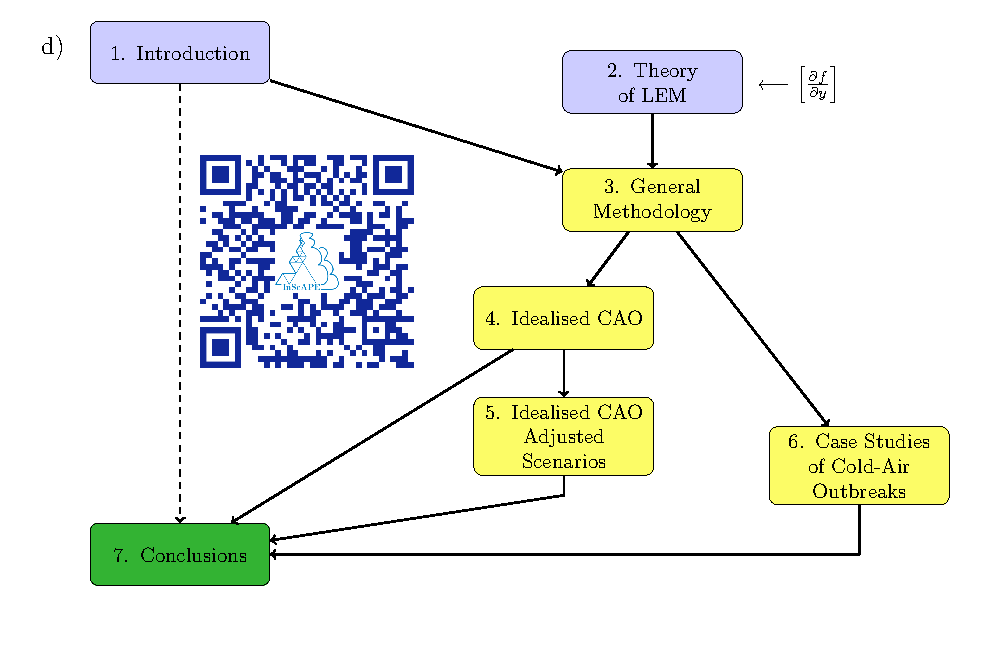
\includegraphics[width=0.7\textwidth]{./figures/standalone.pdf}
        \caption[Diagrams and plots]{Here we combine a \textbf{Tikz} diagrams and images. We can also compile the figure as separate \textbf{standalone} \index{standalone} pdf and then include it as a graphical element. }  
      \label{fig:standalone}
 \end{figure}
 
 %\setcounter{subsection}{7}
 \section{Counters}\label{sec:counters}
How did we suddenly jump from section \ref{sec:figures} to \ref{sec:counters}  ?

 \newpage 
 
 \section{Customizing Links, References, and Citations}
 Such as modifying the style of links to other parts of the same document (\nameref{sec:automatic}) and links to \href{https://geomet.uni-koeln.de/en/}{external websites}.
 
 
 \section{Version Control and Comparison}
 We also look at the \index{tool!external} external tools such as \texttt{latexdiff} that compares two \LaTeX files, and  \texttt{pdfdiff} that compares \( \ldots \) you know what.  
  


  
  
  
  
  
\chapter{Wednesday} \label{chap:wednesday}

 

We will start with:
\input{./data/sillytext1.txt}  
%\input{./data/sillytext2.txt}

\section{Guidelines}
To speed up today the progress of the workshop today, the new commands are not only listed in the text but also included as comments. To make the commands actives, just remove or add comment signs.

\section{External tools}
First we will have a quick look at the \emph{latexdiff} tool from the last time.
But this time, we will  show its shortomings. First, look at the beginning of today chapter and swap which lines are commented between  \texttt{sillytext1.txt} and \texttt{sillytext2.txt}\\
Secondly, open your shell, change to the folder with this file and type \stepcounter{samplecode} (example \alph{samplecode}): 

\begin{lstlisting}[language={bash}, frame=single,basicstyle=\footnotesize]
  latexdiff day2latex.tex day2latex_v2.tex > different.tex
\end{lstlisting}~\vspace{1ex}
\stepcounter{samplecode}

and then compile the output file. Does it highlight any differences?\\

Fortunatelly there is a way to show the differences in the included files. Use the option \texttt{--flatten} which merges all the \texttt{input} files before comparing \stepcounter{samplecode} (example \alph{samplecode}):
\begin{lstlisting}[language={bash}, frame=single,basicstyle=\footnotesize]
  latexdiff --flatten  day2latex.tex day2latex_v2.tex > differentshow.tex
\end{lstlisting}~\vspace{1ex}

We can also play with the style of the latexdiff file. \\


And with the option \texttt{--type}, we can also define how the changes appear. The two most useful choices are:
\begin{itemize}
 \item UNDERLINE --- the added text is not only blue, but also underlined 
 \item PDFCOMMENT --- changes are not marked in the text, but as PDF comments! 
\end{itemize}

Go ahead and give it a try \stepcounter{samplecode} (example \alph{samplecode}):

\begin{lstlisting}[language={bash}, frame=single,basicstyle=\footnotesize]
  latexdiff --flatten --type=PDFCOMMENT day2latex.tex day2latex_v2.tex > differentcom.tex
\end{lstlisting}~\vspace{0ex}

\subsection{Other tools}

There are a couple of other tools that can speed up your work with latex.
Unfortunately they are not installed here. But you can try them later:
\begin{itemize}
    \item \emph{pdfgrep} --- similar to grep, searches inside a PDF document that was already compiled; See: \href{https://www.geeksforgeeks.org/pdfgrep-command-in-linux/}{tutorial},  \href{https://pdfgrep.org/doc.html}{man page}
    \item \emph{pdftk} --- tool for splitting, combing and mixing pdf documents; See: \href{https://www.pdflabs.com/docs/pdftk-cli-examples/}{pdft examples}
\end{itemize}
%-> add links 


\section{Fillers}
 \subsection{Filler text}
 Sometimes we need to test whether the structure of the document and the formatting works. Instead of spending time copying and pasting random stuff, we use the \emph{Lore Ipsum} generator.
In the header we already inserted \texttt{lipsum} package, and here we insert the following command \stepcounter{samplecode}(example \alph{samplecode}):
\begin{lstlisting}[language={[latex]tex}, frame=single,basicstyle=\footnotesize]
  \lipsum[0-2]    %generates dummy text
\end{lstlisting}
%\lipsum[0-2]    % lore ipsum 


\section{Code Listing with Highligths}
You have already seen example of code listing in the previous paragprahs. Now we will look at this topic in more detail.
With teh package \textbf{listings}, you can show the structured code and highlight parts of it. The location of the code could be:
\begin{itemize}
 \item Directly copy and paste to the latex document \ref{code:python}.
 \item You point to the source code file.
 \begin{itemize}
  \item[\(\circ\)] You can event point to the source code of this very file (see \ref{code:thislatex}).
 \end{itemize}
\end{itemize}

\setcounter{lstlisting}{\value{samplecode}}
\refstepcounter{samplecode}
\begin{lstlisting}[language={python},caption={Copy and paste code (example \alph{samplecode})},label={code:python}, 
     frame=single, captionpos=b, basicstyle=\footnotesize\color{cyan},showstringspaces=false, 
     keywordstyle=\color{magenta}, stringstyle=\color{brown}, commentstyle=\color{ForestGreen} 
     ]
 lname = "LaTeX"     # strings brown, comments in dark green
 print("Do you sometimes use {} to generate {} files?".format("Python",lname))
\end{lstlisting}

\refstepcounter{samplecode} 
\lstinputlisting[ language={[latex]tex},      % tex syntax, latex option
  caption={Self-showing code (example \Alph{samplecode})}, label={code:thislatex}, 
  firstline=371, firstnumber=371, lastline=387, numbers=left, captionpos=b,
  breaklines=true, basicstyle=\scriptsize\color{darkgray}, frame=single,
  keywordstyle=\bf\color{magenta}, commentstyle=\color{ForestGreen}  % comments in different colour
]{./day2latex.tex}   % this exact file
% {day2latex_backup.tex}   % alternative code location

\noindent You can try it yourself:
\begin{enumerate}
 \item Change colour which highlights keywords.
 \item Change the comments fonts to italics (hint: \texttt{\textbackslash it})
 \item Adjust the path to the code so it is listing part of this file that your are working on.
\end{enumerate}

\subsection{Callback to Monday}
\begin{enumerate} 
 \item Make the symbol after the word ``example'' in \ref{code:thislatex} is consitent with the rest of examples. 
 \item Instead of the \emph{listing} counter is starts with the value of the \emph{example} counter, make it that the \emph{example} counter being (re)set to the value of the \emph{listing} counter.
 \item Recompile and look how it appears on the page \pageref{listings}
\end{enumerate}

\subsection*{Further Reading}
\addcontentsline{toc}{subsection}{Further Reading}
\begin{itemize}
 \item \href{https://www.overleaf.com/learn/latex/Code_listing}{Overleaf Guidelines on code listings.}
 \item \href{https://nasa.github.io/nasa-latex-docs/html/examples/listing.html}{NASA code listing examples}
 \item \href{https://texdoc.org/serve/listings.pdf/0}{Documentation of Listing Package}
\end{itemize}


\newpage 

\section{Tables}

Sometimes we directly write a table in the latex document. But sometimes we need values from and external file. Shall we just copy and paste them?~\vspace{2ex}\\
Sure, if you want to risk messing up the whole document and losing the newest values.~\vspace{2ex}

\noindent
A better solution is to export the table in a separate file and just input here, such as:
\refstepcounter{samplecode} 
\begin{lstlisting}[language={[latex]tex}, frame=single,basicstyle=\footnotesize]
  \input{/somefolder/exported_table.tex}
\end{lstlisting}

\noindent
But there are even some more comfortable solutions.

\subsection{Importing Tables} \label{sec:tables}
Instead of copy \& paste values into tables, we just read them from an external csv file and format them.  

\refstepcounter{samplecode} 
\lstinputlisting[ language={[latex]tex},      % tex syntax, latex option
  caption={Importing from csv file (example \alph{samplecode})}, label={code:csvimport}, 
  firstline=439, firstnumber=439, lastline=457, numbers=left, captionpos=b,
  breaklines=true, basicstyle=\scriptsize\color{darkgray}, frame=single,
  keywordstyle=\bf\color{magenta}, commentstyle=\color{olive}  % comments in different colour
]{./latex/day2latex_backup.tex}   % 
\begin{table}[h!] \label{tab:import}
  \begin{center} 
  \csvreader[
      tabular = |r|r|r|, 
      table head  = \hline 
          \( \quad  z \; \lbrack \mathrm{m} \rbrack  \) 
          &  \(  \; \bar{u} \;  \lbrack \mathrm{m\, s}^{-1} \rbrack \)
          & \(  \quad \quad \Big. \bar{ \theta }  \; \lbrack \mathrm{K} \rbrack \Big. \) 
          \\
          \hline ,
      table foot = \hline 
          & \multicolumn{2}{ c|}{\( \ldots \) } 
          \\ \hline
  ]{./data/values.csv}  % table location
  {  z=\zvec, u=\uvec, theta=\thvec    % mapping of columns
  }{%
     \zvec  & \uvec & \thvec        % which columns to show
  } % 
  \caption[short table description]{This is a table imported from the csv file. Apart from that this caption is way to long to be shown in the list of tables. And we will also further style-up the table. }
  \end{center}
\end{table} ~\vspace{1ex}

\subsection{Modifying Number Formats}

\newpage 
\subsection{Table Styling}

  We can easily add additional cells to the table.
  
  \begin{table}[h!] \label{tab:styled}
  \begin{center}
  \csvreader[
      tabular = |r|r|r|, 
      table head  =
          %\hline 
          \multicolumn{1}{ c }{ ~}
          & \multicolumn{2}{|c|}{ measured } \\
          \hline 
          \( \quad  z \; \lbrack \mathrm{m} \rbrack  \) 
          &  \(  \; \bar{u} \;  \lbrack \mathrm{m\, s}^{-1} \rbrack \)
          & \(  \quad \quad \Big. \bar{ \theta }  \; \lbrack \mathrm{K} \rbrack \Big. \) 
          \\
          \hline  ,
      table foot = \hline \hline    % doubled horizontal line
         \multicolumn{1}{|c|}{\( \ldots \) }
          & \multicolumn{2}{ c|}{\( \ldots \) } 
          \\ \hline
  ]{./data/values.csv}  % table location
  {  z=\zvec, u=\uvec, theta=\thvec    % mapping of columns
  }{%
     \zvec  & \uvec & \thvec        % which columns to show
  } % 
  \caption[short table description]{This is a table imported from the csv file. Apart from that this caption is way to long to be shown in the list of tables. And we will also further style-up the table. }
  \end{center}
\end{table} ~\vspace{1ex}
  
  What else would you like to modify in the table?


\section{Macros}
We can very much speedup work in \LaTeX with macros --- simple scripts and aliases that speed-up the work.

If we repeatedly write a complicate math expression or symbol, such as
\[ \theta^{\scriptscriptstyle \mathrm{(ML)}} =  \]
we can define it as a macro (in the preamble of the documents)

\stepcounter{samplecode}(example \alph{samplecode}):
\begin{lstlisting}[language={[latex]tex},
    frame=single,basicstyle=\footnotesize]
      \newcommand{\thml}{                        % macro name 
      \theta^{\scriptscriptstyle \mathrm{(ML)}}  % inner code
  }                                              % close brackets
\end{lstlisting}
and then just output \( \thml \) by calling the macro:
\begin{lstlisting}[language={[latex]tex},
    frame=single,basicstyle=\footnotesize]
     \thml
\end{lstlisting}
\index{macro@{\bf{macro definition}}}
Try to define a macro for your favourite math symbol and use it! \\

\subsection{Macro Arguments}
\index{macro!argument}
Macros can also take a number of arguments, here for example 3, with the first two being optional and predefined. You can see in the preable of this documents:

\refstepcounter{samplecode} 
\lstinputlisting[ language={[latex]tex},      % tex syntax, latex option
  caption={Macro with arguments (example \alph{samplecode})}, label={code:macroarg}, 
  firstline=141, firstnumber=141, lastline=143, numbers=left, captionpos=b,
  breaklines=true, basicstyle=\scriptsize\color{darkgray}, frame=single,
  keywordstyle=\bf\color{magenta}, commentstyle=\color{olive}  % comments in different colour
]{./latex/day2latex_backup.tex}   

And then you call it:
\begin{lstlisting}[language={[latex]tex},
    frame=single,basicstyle=\footnotesize]
     \sayabout[rude]{person}{Jan}
\end{lstlisting}
which outputs: \sayabout[rude]{person}{Jan}.\\

\noindent
Let us play with this macro: \index{macro!argument!optional}
\begin{enumerate}
 \item Call it without the optional argument from the call. 
 \item Call it with changed arguments. 
\end{enumerate}

\subsection{Redefing Macros}
Not only we can define new macros, but we can \emph{carefully} redefine them using the \texttt{\textbackslash renewcommand}.\\

\begin{enumerate}
 \item Look at the title at the page \pageref{contents}
 \item Search in the preamble for \texttt{\textbackslash renewcommand} and change it to something meaningful.
 \item Try to redefine some other macro. 
\end{enumerate}


\subsection{More on Macros} 
 We can also write conditional macros which allows us to say IF something, THEN do something, ELSE do something else. For that we would use package \texttt{ifthen} and call it:
 

\begin{lstlisting}[language={[latex]tex},
    frame=single,basicstyle=\footnotesize]
    \ifthenelse{\equal{\thing}{\string whatever}}
    {% True case
      \newcommand{\result}{thing is `whatever'.}%
    }
    {% false case
      \newcommand{\result}{thing is something else.}%
    }
 \end{lstlisting}
 
 We can even use \texttt{foreach} command from the package \texttt{tikz}. This is particularly useful for drawing repeated patterns.
 
\section{Index Page}
Index is a very popular part of books and longer documents.
To generate it, we need to use the package \texttt{makeidx} in the preamble and the command 
\begin{lstlisting}[language={[latex]tex},
    frame=single,basicstyle=\footnotesize]
     \makeindex
\end{lstlisting}
also in the premable. You can see the result on the following page:


% ---  index--------------
  \clearpage
  \phantomsection                       % to keep good formatting 
  \addcontentsline{toc}{subsection}{Index Page Itself} 
  \label{index}  
  \printindex   
%-------------------------
   
  \subsection{Tasks for the Index}
  \begin{enumerate}
   \item Looks up examples of index entries in this document.
   \item Add some with subentries. 
   \item Modify the style of some of them.
  \end{enumerate}

  
\section{Formatting} 
\subsection{Dashes}
Dash is not the same thing as minus. 
Lets see the difference between following symbols:\\
- \\
-- \\
--- \\
 
 \section{Posters and Slideshows} 
 If you have been struggling with Powerpoint, there is a way out \( \ldots \) 
 

 




\newpage
\label{LastPage}
\begin{center}
 The end
\end{center}



\end{document}
